\documentclass[a4paper]{article}


\usepackage[
    style=numeric, 
    backend=biber, 
    sorting=none
]{biblatex}
\usepackage{graphicx}
\usepackage{enumitem}
\usepackage{geometry}
\usepackage{sectsty}
\usepackage{indentfirst}
\usepackage{times}
\usepackage{listings}

\setlist{
  listparindent=\parindent,
  parsep=0pt,
}

% code block style
% -- Defining colors:
\usepackage[dvipsnames]{xcolor}
\definecolor{codegreen}{rgb}{0,0.6,0}
\definecolor{codegray}{rgb}{0.5,0.5,0.5}
\definecolor{codepurple}{rgb}{0.58,0,0.82}
\definecolor{backcolour}{rgb}{0.95,0.95,0.92}% Definig a custom style:
\lstdefinestyle{mystyle}{
    backgroundcolor=\color{backcolour},   
    commentstyle=\color{codepurple},
    keywordstyle=\color{NavyBlue},
    numberstyle=\tiny\color{codegray},
    stringstyle=\color{codepurple},
    basicstyle=\ttfamily\footnotesize\bfseries,
    breakatwhitespace=false,         
    breaklines=true,                 
    captionpos=t,                    
    keepspaces=true,                 
    numbers=left,                    
    numbersep=5pt,                  
    showspaces=false,                
    showstringspaces=false,
    showtabs=false,                  
    tabsize=2
}% -- Setting up the custom style:
\lstset{style=mystyle}

\sectionfont{\centering}
\addbibresource{citation.bib}
\graphicspath{{./images/}}
\geometry{a4paper, top=4.0cm, bottom=3.0cm,
          left=4.0cm, includehead, includefoot}
\renewcommand\contentsname{Daftar Pustaka}
\emergencystretch=2em

\begin{document}
\linespread{1.5}

\title{Marketplace For Hobby}
\author{Aldih Suhandi, Chandra Wijaya, Ibrahim Seto Aditama}

\maketitle
\begin{figure}[h]
    \centering
    
\includegraphics[width=10cm]{logo_binus.png}\\
    Binus University\\
    2022
\end{figure}
\begin{figure}[h]
    \centering
    Diperiksa Oleh**\\
    \vspace{15mm}
    \begin{tabular}{@{}p{2.5in}@{}}
    \centering
    Nama Dosen - Kode Dosen
    \end{tabular}
\end{figure}

\newpage
\addcontentsline{toc}{section}{\protect\numberline{}Daftar Pustaka}
\tableofcontents

\newpage
\section*{Pendahuluan}
\addcontentsline{toc}{section}{\protect\numberline{}Pendahuluan}

Perkembangan teknologi yang pesat telah melahirkan banyak teknologi baru yang dapat membantu dan mempermudah kita manusia dalam menjalankan kehidupan dan melaksanakan tugas dan keinginan kita. Dari perkembangan teknologi tersebut yang memiliki dampak yang cukup tinggi adalah internet, yang dimana di negara Indonesia ini internet mendapatkan peningkatan popularitas yang dapat diukur dengan peningkatan pengguna internet tersebut dalam tiap tahun, Menurut survey yang diadakan oleh Asosiasi Penyelenggara Jasa Internet Indonesia (APJII) di tahun 2017 perkembangan pengguna internet dari tahun 2016 ke tahun 2017 memiliki pertambahan sebesar 10.56 juta (disurvey pada 2016 ada 132.7 juta dan di 2017 ada 143,26 juta)\autocite{indonesia2017infografis}.


Dari penggunaan internet, kegiatan usaha jual/beli barang yang dilakukan secara text/chat ataupun melalui \textit{e-commerce} merupakan kegiatan yang cukup populer saat memanfaatkan internet dimana di Indonesia di survey APJII pembelian barang memiliki 32.19\% dan jual barang 8.12\% pada layanan yang diakses ketika mengakses internet\autocite{indonesia2017infografis}. \textit{Platform} untuk mempermudah usaha kegiatan jual/beli barang dilengkapi fitur \textit{search} yang cukup, dimana barang dapat dicari dan ditemukan melalui mencari namanya atau menelusuri kategori dari barang tersebut. Kegiatan beli barang dapat untuk mendapatkan barang baku, kebutuhan sehari-hari dan lain-lain. Kategori barang yang menjadi perhatian dan sorotan kami adalah barang berhubungan dengan hobi dimana yang mengalami peningkatan popularitas belakangan ini oleh karena pandemi\autocite{langstedt2022loneliness}.


Oleh karena itu kami melakukan survei untuk mengetahui tentang apa yang mungkin menjadi kesulitan dalam membeli barang terkait hobi di aplikasi \textit{e-commerce}, yang dimana kami mendapatkan bahwa untuk pertanyaan kami “Apakah anda takut untuk mengambil hobi baru karena tidak tau mulai dari mana?” memiliki respon 66.7\% menjawab iya, dan juga pda pertanyaan berhubungan mengenai kesulitan untuk memilih barang yang cocok memiliki respons ya pada persentase yang diatas 50%.


Dari latar belakang tersebut, dimana dalam membeli sebuah barang hobi terjadi keraguan/kesulitan dalam memilih barang yang cocok untuk memulai atau membeli yang cocok, tujuan dari proyek ini adalah untuk mengajukan sebuah sistem aplikasi jual/beli barang khusus dan terfokus mengenai Hobi-hobi dimana barang yang dijual selain dapat diberi kategori, barang juga dapat diberikan dua penilaian tingkat peminatan dalam hobi tersebut sebagai filter tambahan, kita beri nama \textit{Interest Level}, penilaian tersebut diberikan oleh penjual dan juga nanti diberi oleh pembeli sebagai validasi apakah pemberian penilaian tersebut sesuai atau tidak dan juga karena ini sebuah aplikasi untuk hobby, ada sebuah forum untuk melakukan diskusi dengan cara membuat post mengenai kategori hobi yang diinginkan.

\newpage
\section*{Tinjauan Pustaka}
\addcontentsline{toc}{section}{\protect\numberline{}Tinjauan Pustaka}
% OOP, Functional Programming, Design Pattern, Architecural Pattern

\begin{enumerate}
    \item \textit{Object Oriented Programming}

    \textit{Object Oriented Programming} adalah konsep programming yang berdasarkan \textit{objects}, sebuah \textit{object} adalah sesuatu entitas yang ada didunia nyata yang bisa diindetifikasi secara unik\autocite{liang_liang_2021}. Sebagai contoh, sebuah meja, seorang guru, dan bahkan hutang bisa dijadikan sebagai \textit{object}. 

    Untuk membuat sebuah \textit{object} diperlukan sebuah \textit{template} atau \textit{blueprint}, \textit{template} atau \textit{blueprint} ini dalam \textbf{OOP} disebut sebagai \textit{class}, secara definisi \textit{class} adalah sebuah \textit{blueprint} yang dipakai untuk membuat sesuatu atau \textit{object} yang lebih spesifik atau konkrit\autocite{education-erin-oop-2020}, \textit{class} biasanya hanya menampung atribut - atribut yang secara general, seperti tinggi, berat badan, umur, dan sebagainya. Sedangkan sebuah \textit{object} akan menampung \textit{value} yang lebih spesifik, seperti \textit{object} tersebut bertinggi 2 meter dan \textit{object} sudah berumur 3 tahun.

    \textbf{OOP} memiliki 4 pilar pendukung, yaitu:
    \begin{itemize}

        \item \textit{Encapsulation}

        \textit{Encapsulation} adalah konsep dimana semua atribut atau fitur yang ada didalam \textit{object} itu tidak bisa dilihat dan diubah oleh \textit{object} lain, kecuali akses tersebut didefinisikan secara explicit\autocite{education-erin-oop-2020}. Sebagai contoh, \textit{object} manusia memiliki tanggal lahir, karena tanggal lahir itu pasti tidak bisa diubah, atribut tanggal lahir dari \textit{object} tersebut hanya bisa dibaca oleh \textit{object} lain tapi tidak bisa diubah.
        
        Kohesi, konsistensi, dan enkapsulasi adalah pedoman yang baik untuk mencapai sebuah design yang jelas. Sebuah \textit{class} harus memiliki kontrak yang jelas yang mudah dijelaskan dan dipahami, seperti atribut apa saja yang bisa diakses dan diubah oleh \textit{object} atau \textit{class} lain\autocite{liang_liang_2021}.

        \begin{figure}[h]
            \centering
            \begin{lstlisting}[language=Java]
public class Human {
    private Date dateOfBirth;

    public Date getDateOfBirth() {
        return this.dateOfBirth;
    }
}\end{lstlisting}
            \caption{Contoh dari \textit{encapsulation}}
        \end{figure}

        \item \textit{Abstraction}

        \textit{Abstraction} dan \textit{encapsulation} adalah dua sisi dari koin yang sama, \textit{encapsulation} adalah konsep untuk mengatur akses suatu atribut, kalau \textit{abstraction} adalah \textit{class} lain tidak perlu tahu bagaimana \textit{class} ini melakukan suatu tugas\autocite{liang_liang_2021}. Sebagai contoh, saat merakit komputer, kalian hanya tau komponen - komponen didalam komputer itu apa saja, untuk merakit komputer tersebut kalian hanya perlu tau apa saja peran dari tiap komponen yang ada, tidak perlu mengetahui untuk melaksanakan peran mereka, apa yang mereka harus lakukan.
        \newpage
        
        \item \textit{Inheritance}

        \textit{Inheritance} adalah sebuah konsep dimana \textit{class} dapat mempunyai atribut dan fitur turunan dari \textit{class} lain. \textit{Class} yang mendapat fitur turunan ini disebut \textit{child class}, sedangkan \textit{class} yang diturunkan disebut \textit{parent class}\autocite{education-erin-oop-2020}. 

        Tujuan dari konsep ini adalah untuk mengurangi redudansi sebanyak mungkin, dengan cara mengeneralisasikan beberapa \textit{class}, karena beberapa \textit{class} yang berbeda bisa saya memiliki fitur atau atribute yang sama. Sebagai contoh \textit{class} guru, murid, dan kepala sekolah memiliki beberapa atribut yang sama, seperti tinggi badan, berat badan, dan umur. Semua atribut yang sama tersebut bisa dijadikan sebuah \textit{parent class} yang bernama \textit{human} dan \textit{class} guru, murid, dan kepala sekolah akan menjadi \textit{child class} dari \textit{class} tersebut\autocite{liang_liang_2021}.

        \begin{figure}[h]
            \centering
            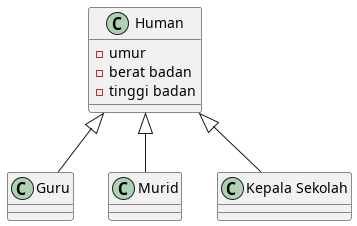
\includegraphics[width=8cm]{inheritance example.png}
            \caption{Contoh dari \textit{inheritance}}
        \end{figure}

        \item \textit{Polymorphism}

        \textit{Child class} adalah sebuah \textit{class} yang akan menuruni semua atribut dan fitur dari \textit{parent class}, tapi apabila dari satu \textit{parent class} memiliki 2 \textit{child class} yang memiliki fitur yang sama tapi cara melakukannya yang berbeda? contoh pisang goreng adalah sebuah makanan, tapi tidak semua makanan adalah pisang goreng, ada perubahan dari cara memasak dan cara penyajian ditiap - tiap makanan, disini konsep \textit{polymorphism} dapat dipakai. Secara definisi \textit{polymorphism} adalah kelakuan dimana \textit{child class} bisa melakukan suatu \textit{task} atau fitur yang sama seperti \textit{parent class} dengan cara yang berbeda\autocite{education-erin-oop-2020}.
    \end{itemize} 

    
    \item \textit{Funtional Programming}
    
    \textit{Functional Programming} adalah sebuah konsep, paradigma atau sebuah macam \textit{software development} yang menekankan titik beratnya pada penggunaan \textit{functions}, \textit{Functional Programming} sendiri bukan merupakan sebuah alat yang dapat digunakan tetapi merupakan sesuatu pegangan untuk \textit{developers} sebagai sebuah cara menulis kode\autocite{atencio2016functional}.


    Tujuan dari \textit{Functional Programming} adalah membuat sebuah \textit{function} yang lebih kecil yang memiliki sifat dapat digunakkan kembali, lebih dapat diandalkan dan mudah dimengerti, lalu \textit{functions} tersebut maka akan dapat membuat sebuah program yang lebih dapat dimengerti \autocite{atencio2016functional}. \textit{Function} yang dibuat mengikuti \textit{Functional Programming} biasa dibuat dengan melakukan parameterisasi pada \textit{function} supaya dalam menggunakannya dengan menggunakkan parameter kode tersebut dapat digunakkan kembali untuk melakukan hal yang lain. \textit{Functional Programming} memiliki empat konsep dasar, yaitu \textit{Declarative programming}, \textit{Pure functions}, \textit{Referential transparency}, dan \textit{Immutability}\autocite{atencio2016functional}.


    \begin{itemize}
        \item \textit{Declarative programming} adalah sebuah pendekatan \textit{programming} dimana sebuah kode untuk melakukan sesuatu akan ditulis menggunakan \textit{expressions} yang mendeskripsikan logika dari suatu program. Berbeda dengan Imperatif atau \textit{Procedural Programming} dimana akan ditulis secara detail bagaimana untuk melakukan sesuatu untuk mencapai hasil yang diinginkan\autocite{atencio2016functional}. 
        \item \textit{Pure functions} adalah \textit{function} yang memiliki dua sifat, yaitu pertama, sebuah pure function hanya dan hanya bergantung pada input yang diberikan dan tidak dengan \textit{state} yang tersembunyi dan/atau external (diluar function tersebut) dan kedua, tidak merubah apapun yang diluar dari \textit{function} tersebut seperti obyek global atau parameter yang di \textit{pass} ke \textit{function} tersebut \autocite{atencio2016functional}. 
        \item \textit{Referential transparency} adalah ketika sebuah \textit{function} menghasilkan hasil yang sama juga diberikan input yang sama \autocite{atencio2016functional}.
        \item \textit{Immutability} adalah dimana dalam \textit{Functional Programming} untuk melestarikan sebuah data supaya \textit{Immutable} tidak bisa diganti setelah di deklarasi. Dalam konsep ini yang perlu diperhatikan adalah object seperti \textit{array} yang dapat berubah konten atau valuenya dalam sebuah function \autocite{atencio2016functional}.  
    \end{itemize}

\end{enumerate}

\newpage
\section*{Metode Pelaksanaan}
\addcontentsline{toc}{section}{\protect\numberline{}Metode Pelaksanaan}

\subsection*{\textit{Tech Stack}}
\addcontentsline{toc}{subsection}{\protect\numberline{}\textit{Tech Stack}}
\begin{enumerate}
    \item \textit{Back end} 

    \textit{Back end} atau bisa disebut juga \textit{developer's end} adalah sebuah layer yang memproses semuanya dibelakang layar dan tempat terjadinya sesuatu yang tidak bisa dilihat oleh \textit{user}\autocite{letsgodojo-frontend-backend}. Analogy yang bisa digunakan adalah saat disebuah restoran ada pelanggan yang memesan sesuatu yang spesifik ke pelayan, ini adalah bagian \textit{front end} dari restoran tersebut, setelah itu pelayan memberikan pesanan tersebut ke koki, yang akan mengambil bahan masak, momotong semua bahan - bahan tersebut, dan memasaknya sesuai resep yang sudah dibuat, koki ini yang merepresentasikan bagian \textit{backend} dari restoran tersebut\autocite{codecademy-backend}. 

    \textit{Back end} terdiri dari dua hal, \textit{servers} yang akan meproses data dan \textit{request} dari sebuah user dan \textit{database} yang akan menyimpan data yang sudah atau yang akan mau diproses\autocite{codecademy-backend}. Dalam proyek ini, kami akan menggunakan \textit{springboot} sebagai \textit{framework} yang digunakan untuk membuat \textit{software back end}-nya dan \textit{\textbf{MySQL}} sebagai database yang digunakan.

    \textit{Springboot} adalah \textit{java back end framework} yang paling populer didunia, \textit{springboot} membuat menulis \textit{software back end} menjadi lebih mudah dan lebih cepat\autocite{spring-framework}, alasan kenapa kami menggunakan \textit{springboot} adalah sebagai berikut:
    \begin{itemize}
        \item \textit{Springboot} mempunyai banyak \textit{plugin} yang dapat di\textit{install};
        \item komunitas \textit{springboot} itu sangat besar;
        \item dan yang terakhir \textit{springboot} memiliki fitur \textit{Inversion of Control} dan \textit{Dependency Injection}.
    \end{itemize}

    \item \textit{Front end}
\end{enumerate}
% mysql
% springboot
% reactjs base framework
% payment API TODO: aldih

\subsection*{System Architecture}
\addcontentsline{toc}{subsection}{\protect\numberline{}System Architecture}
% sequence diagram secara general
% mock up aplikasi

\subsection*{Aplikasi Serupa}
\addcontentsline{toc}{subsection}{\protect\numberline{}Aplikasi Serupa}
% bikin table
% buat +- dari aplikasi serupa ini

\subsection*{Pengumpulan Data Pengguna}
\addcontentsline{toc}{subsection}{\protect\numberline{}Pengumpulan Data Pengguna}

\newpage
\addcontentsline{toc}{section}{\protect\numberline{}Referensi}
\printbibliography[title=Referensi]

\end{document}
